\chapter{Relatedness and Similarity}
In Chapter~\ref{chap:theory}, I laid out the theoretical groundwork for statistical context sensitive models of lexical semantics, and in Chapter~\ref{chap:method} I described the actual methodology for building such models, accompanied by a preliminary proof of concept involving conceptual entailment.  In this chapter, I will present the first set of experiments designed to evaluate the utility of this methodology.  These experiments are intended to probe the productivity of a context sensitive, geometric approach to building a computational model of lexical semantics based on statistics about word co-occurrences.  Beyond testing my models' performances on some well-travelled datasets, this will provide an opportunity to explore whether different components of the methodology and, moreover, different aspects of geometric output lend themselves to modelling related but distinct semantic phenomena.

So, moving into familiar computational linguistic territory, I will explore my methodology's performance on two different phenomena: \emph{relatedness} and \emph{similarity}.  Each of these objectives have provided reliable but distinct evaluative criteria for computational models of lexical semantics.  One of the hypotheses I will put forward regarding my methodology is that the geometrically replete subspaces generated by my contextualisation techniques should provide features for the simultaneous representation of related, diverse, and sometimes antagonistic aspects of language.  Experimenting with these established datasets will provide a platform for exploring the ways in which different features of a semantic structure projected into one of my contextualised subspaces shift as the relationships inherent in the generation of the subspace likewise change, and this will in turn lead to some searching questions about the importance of context in the computational modelling of these particular semantic phenomena in the first place.

A fundamental objective for a general semantic model is a mechanism for measuring the relatedness inherent in semantic representations.  The distributional hypothesis itself is framed in terms of the relatedness between words: if words that tend to have a similar co-occurrence profile should also tend to have similar meaning, then, in some sense of the word, \emph{similarity} is what is being captured by the word-vectors that populate a distributional semantic model.  There is, however, an ambiguity at play in terms of what exactly it means for two words to denote things that are semantically \emph{related}, and when this designation should include the more specific category of \emph{similarity} (or, for that matter, other types of relatedness such as \emph{meronymy}, \emph{analogy}, even \emph{antonymy}, and so forth).  So, for instance, the words \emph{tiger}, \emph{claw}, \emph{stripe}, \emph{ferocious}, and \emph{pounce} are all clearly related in the way that they trace out aspects of a very specific conceptual space of \textsc{tigerness}, but none of them are similar in the way that \emph{tiger}, \emph{lion}, and \emph{bear} are all commensurable constituents of a space of \textsc{wild animals}.

The compilation of data for the purpose of testing the ability of computational models to identify semantic relationships between words has tended to focus on the general case of relatedness rather than more nuanced similarity, if sometimes simply through a failure to specify between the two.  The methodology for generating this data goes something like this: human participants are given a set of pairs of words and asked to quantify, for instance, the ``similarity of meaning'' \citep[][p. 628]{RubensteinEA1965} in each pair, or ``how strongly these words are related in meaning,'' \citep[][p. 124]{YangEA2006}.  \cite{FinkelsteinEA2002} use both the terms \emph{similarity} and \emph{relatedness} in the instructions for generating their WordSim353 data, analysed below, ultimately asking evaluators to rank words from being ``totally unrelated'' to ``very related'';\footnote{Copies of the instructions, along with the data itself, can be found at \url{www.cs.technion.ac.il/~gabr/resources/data/wordsim353/wordsim353.zip}.} \cite{BruniEA2012} used only the term \emph{relatedness} in their instructions, with no mention of \emph{similarity}.\footnote{Instruction and data are at \url{https://staff.fnwi.uva.nl/e.bruni/MEN}.}  \cite{FaruquiEA2016} have discussed the uncertainty inherent in human ratings produced in this manner, pointing out that judgements of similarity and relatedness can be subjective and task specific.

Relatively recently, researchers have made a concerted effort to generate data that focusses on word similarity specifically, rather than a less clearly defined notion of relatedness.  \cite{AgirreEA2009} have taken the widely used WordSim data and split it into two overlapping sets of word pairs, one intended to reflect a range of judgements on word similarity and the other judgements on relatedness, based on human evaluations of the types of relationships inherent in each word pair.  Subsequently \cite{HillEA2015} have created Their SimLex999 dataset by extracting word pairs from an existing set of word associations, sampling from a range of conceptual relationships, and then giving human evaluators detailed instructions casting similarity in terms of degree of synonymity.  These datasets have proven more resistant to highly accurate modelling through standard distributional semantic approaches---indeed, an interesting corollary to the distinction between relatedness and similarity has been the development of \emph{knowledge based} versus \emph{corpus based} techniques for modelling these semantic phenomena \citep[see][for a discussion]{MihalceaEA2006,HassanEA2011}, with corpus based, or statistical, techniques proving more suited to modelling relatedness rather than similarity.

My thoroughly statistical methodologies will be initially tested on the WordSim data in order to explore my subspaces' capacities for capturing semantic relatedness and the SimLex data in order to explore how it handles similarity.  Results for each dataset will be examined in turn, first exploring the way that human ratings can be fit to full sets of geometric features using linear models, then examining the correlation between independent features and human ratings, and finally exploring ways to learn combinations and features that should be generally predictive of the phenomena under examination.  The most valuable outcome of this set of experiments, however, will be the comparison between the models learned for each of these related but distinct semantic phenomena, and in particular an analysis of the geometric features of subspaces which correlate with different measures of the conceptual interrelations between lexical representations.  This meta-analysis will serve to test my hypothesis that different statistical features of an appropriately contextualised semantic space map to different semantic phenomena, and the corresponding claim that context sensitive representations can capture various semantic features as dynamic properties in a single subspace.  Finally, the analysis of the different geometric correlates of relatedness and similarity lends itself to a consideration of the way in which the frames within which humans evaluate semantic relationships may themselves be contextual.

\section{An Experiment on Relatedness}
Standard distributional semantic models have generally tended to capture semantic relatedness over similarity in terms of the proximity between semantic representations.  This point, evidenced by the stronger results achieved on relatedness tests by statistical models, can be seen clearly by imagining the contexts in which words such as \emph{good} and \emph{evil} or \emph{day} and \emph{night} might be expected to regularly occur: there is no serious case to be made that the meaning of a sentence would not be significantly changed by toggling these word pairs in actual sentences (they are closer to being antonyms than to being synonyms), but it is equally reasonable to guess that these words will generally have similar co-occurrence profiles.  Examples of corpus derived, distributional semantic type models that have performed well on on word relatedness evaluations include the work of \cite{GarbilovichEA2007} and \cite{HassanEA2011}, both of whom have applied vector building techniques that exploit Wikipedia page labels to enhance the conceptual knowledge inherent in their lexical representations.  \cite{HalawiEA2012} similarly enhance neural word embeddings derived from co-occurrence observations with synonymy information extracted from WordNet.  And \cite{LuongEA2013} use recursive neural networks to actually move to a level of linguistic abstraction below the word itself, modelling the morphology and the corresponding composition of words based on morphemes as a productive element in predicting relatedness between words.  The overall import of this literature is that there is scope for using corpus analytic techniques to build lexical representations that do a good job of capturing semantic relatedness.

Nonetheless, there may be some advantages to identifying context specific subspaces based on an analysis of word pair inputs.  For instance in cases where one of the words being compared has multiple senses, the selection of mutually relevant co-occurrence dimensions under the \textsc{joint} and \textsc{zipped} techniques might offer a degree of disambiguation.  Beyond this, I hypothesise that similar measures to the ones that have proved productive for static vector space models, so, in particular, measures of cosine similarity between word-vectors, anchored at the origin as well as at the generic points of the space, should be indicative of semantic relatedness.  I further predict, following on the results reported earlier in this chapter on the relationship between the norm of vectors in contextualised subspaces and conceptual entailment, that measures involving the distance of word-vectors from the origin will also correlate positively with relatedness, and here my subspaces, with their sense of interior and exterior, centre and periphery, should have an advantage.

\subsection{Relatedness: Methodology and Model}
In order to test the ability of my statistical methodologies to likewise model relatedness, I build \textsc{joint}, \textsc{indy}, and \textsc{zipped} subspaces using each of the 353 word pairs in the WordSim data as input.  I project subspaces of 20, 50, 200, and 400 dimensions, extrapolated from base spaces built using 2x2 and 5x5 word co-occurrence windows.  For each subspace, I extract the geometric features listed in the previous chapter in Table~\ref{tab:features} and use these as the independent variables of a linear regression, taking the WordSim rating of the word pair used to generate the subspace as the dependent variable.  The relatedness ordering of word pairs inherent in the scores assigned by the regression are then compared to human WordSim ratings in terms of Spearman's correlations, as is standard practice in the NLP literature.  Results from my model are compared with results from singular value decompositions of my base space using comparable parameters, as well as \texttt{word2vec} skip-gram and bag-of-words models, again using commensurable parameters.

\begin{table}
\centering
\begin{tabular}{lrrrr|rrrr}
\hline
\emph{window} & \multicolumn{4}{c}{2x2} & \multicolumn{4}{c}{5x5} \\
\emph{dimensions} & 20 & 50 & 200 & \multicolumn{1}{c}{400} & 20 & 50 & 200 & 400 \\
\hline
\textsc{joint} & 0.666 & 0.681 & 0.698 & 0.728 & 0.704 & 0.698 & 0.700 & 0.709 \\
\textsc{indy} & 0.671 & 0.676 & 0.702 & 0.707 & 0.703 & 0.712 & 0.715 & 0.729 \\
\textsc{zipped} & 0.642 & 0.674 & 0.699 & 0.698 & 0.652 & 0.678 & 0.716 & 0.717 \\
\textsc{SVD} & 0.521 & 0.618 & 0.690 & 0.728 & 0.527 & 0.663 & 0.722 & 0.742 \\
\textsc{SG} & 0.549 & 0.639 & 0.696 & 0.701 & 0.544 & 0.635 & 0.705 & 0.710 \\
\textsc{CBOW} & 0.557 & 0.648 & 0.700 & 0.695 & 0.584 & 0.663 & 0.716 & 0.716 \\
\hline
\end{tabular}
\caption{Spearman's correlations for word ratings output by a linear regression model of the WordSim data for various subspace types and model parameters, compared to the correlations for cosine similarities output by static models using comparable parameters.}
\label{tab:related}
\end{table}

Results are reported in Table~\ref{tab:related} (and all correlations are statistically significant with $p < .001$).  The first thing to note is that the best performance overall is achieved by the 5x5 word window, 400 dimensional version of the SVD factorisation of my base space (though the difference between this correlation and the slightly lower correlation achieved with the same parameters for the \textsc{indy} dimension selection technique is not significant, with $p = .356$).  More generally, the 5x5 word co-occurrence window versions of all models tend to perform more strongly on this task than the 2x2 versions, suggesting that semantic relatedness is a property of the broader sentential context in which a word occurs rather than just the immediate syntagmatic tendencies of a word.\footnote{\cite{Sahlgren} discusses \citepos{Saussure} semiotic notions of \emph{syntagm} (the way that words are composed into meaningful utterances) and \emph{paradigm} (the way that words are comparable and potentially interchangeable units of meaning) in the context of distributional semantics.}  It is also notable that my context sensitive methods outperform the static models at lower dimensionality (and here the difference is significant, with $p < .005$ in a comparison between the \textsc{joint} 5x5 window, 20 dimensional correlation and the corresponding result for the \textsc{CBOW} model).  It seems that the contextually selected dimensions are initially all more informative about relatedness than the degree of general variance captured in lower numbers of dimensions using either factorisation or neural modelling techniques.

In terms of comparing between my dimensional selection techniques, the \textsc{joint} and \textsc{indy} techniques perform somewhat comparably, with the \textsc{indy} technique doing a bit better in the 5x5 spaces.  The strong performance of the \textsc{joint} technique in the 2x2 models at 400 dimensions seems anomalous.  The joint technique in particular should begin to run out of useful dimensions to select between words as the dimensionality of the spaces scale up, and so would be expected to follow a similar trend as with the \textsc{zipped} subspaces, where results begin to tail off after 200 dimensions---and this effect should be more prominent in the 2x2 models, where there is less overall co-occurrence information available.  It's likewise interesting that the \textsc{zipped} technique offers consistently lower correlations, particularly considering that this technique was conceived as something of a hybrid between the comprehensive \textsc{joint} approach and the independent \textsc{indy} approach.  It would seem, then, that the dimensions most predictive of semantic relatedness are either those which are substantially informative about both words being compared, or those which are highly informative about one word and only incidentally informative about the other, to the exclusion of the middle ground of dimensions that are highly informative about one word and at least marginally informative about another.  The conclusion to draw here is that the \textsc{joint} and \textsc{indy} spaces are identifying relatedness in two different capacities: in the case of the former, the degree of proximity between two points with fairly high values is being captured, while in the case of the latter the extent to which there is some degree of overlap (or, alternatively, the extent of the orthogonality) between the salient co-occurrence features is being exploited.

\subsection{The Geometry of Relatedness}

It must at this point be noted that the models described above are instances of fitting the output produced by my methodologies to human generated ratings, and so they should not be construed in some sense as solutions to the problem of computationally modelling the cognitive processes involved in judging semantic relatedness.

In order to get a sense of what's actually happening in these models, I next produce Spearman's correlations between the WordSim data and each of the features of different subspaces independently.  The top five features for 400 dimension \textsc{joint}, \textsc{indy}, and \textsc{zipped} spaces generated using 2x2 word co-occurrence windows are reported in Table~\ref{tab:ind-related}.  Here a strong correlation between the most predictive of the \textsc{joint} and \textsc{zipped} subspaces is evident, and this makes sense: as these types of subspaces increase in dimensionality, the possible combinations of co-occurrence dimensions with non-zero values for both input word-vectors decreases, so the subspaces themselves begin to converge.  The features selected here tend to involve the mean norm of the input word-vectors, so the prominence of these vectors in the spaces that are jointly informative about both of them is clearly positively correlated with relatedness between the two terms.\footnote{There is clearly a high degree of multicollinearity at play between these top independent features, and this will be addressed below.}  In other words, related words tend to share strong PMI values with a number of co-occurrence dimensions---hardly a surprising finding, and in line with the results indicating the powerfulness of norm measures revealed in the proof of concept outlined earlier in this chapter.

%\begin{table}
%\centering
%\begin{tabular}{lr|lr|lr}
%\hline
%\multicolumn{2}{c}{\textsc{joint}} & \multicolumn{2}{c}{\textsc{indy}} & \multicolumn{2}{c}{\textsc{zipped}} \\
%\hline
%$\mu (A,B)$ & 0.609 & $\angle ACB$ & 0.683 & $\mu (A,B)$ & 0.611 \\
%$\mu (A,B)/C$ & 0.604 & $\angle AMB$ & 0.654 & $\mu (A,B)/X$ & 0.603 \\
%$\mu (A,B)/X$ & 0.603 & $\angle A'C'B'$ & 0.600 & $\mu (A,B)/C$ & 0.598 \\
%$\mu (A,B)/M$ & 0.602 & $\angle AOB$ & 0.594 & $\mu (A,B)/M$ & 0.596 \\
%$\angle ACB$ & 0.574 & $\angle A'X'B'$ & 0.571 & $\angle AMB$ & 0.566 \\
%\hline
%\end{tabular}
%\caption{Independent Spearman's correlations with WordSim data for top five features of each subspace type for 2x2 word co-occurrence window, 400 dimension subspaces.}
%\label{tab:ind-related}
%\end{table}

\begin{table}
\centering
\begin{tabular}{lr|lr|lr}
\hline
\multicolumn{2}{c}{\textsc{joint}} & \multicolumn{2}{c}{\textsc{indy}} & \multicolumn{2}{c}{\textsc{zipped}} \\
\hline
$\angle AMB$ & 0.645 & $\angle ACB$ & 0.721 & $\angle AMB$ & 0.636 \\
$\angle ACB$ & 0.636 & $\angle AMB$ & 0.703 & $\angle ACB$ & 0.607 \\
$\mu (A,B)/M$ & 0.604 & $\angle A'C'B'$ & 0.663 & $\mu (A,B)$ & 0.603 \\
$\mu (A,B)$ & 0.604 & $\angle A'X'B'$ & 0.634 & $\angle A'M'B'$ & 0.593 \\
$\mu (A,B)/C$ & 0.603 & $\angle AOB$ & 0.634 & $\angle A'X'B'$ & 0.587 \\
\hline
\end{tabular}
\caption{Independent Spearman's correlations with WordSim data for top five features of each subspace type for 5x5 word co-occurrence window, 400 dimension subspaces.}
\label{tab:ind-related}
\end{table}

Much more interestingly, though, an altogether different set of top features emerges for the \textsc{indy} subspaces.  Here, angular measures are more predictive of relatedness across the board, with the measure $\angle ACB$, the angle of the word-vector points $A$ and $B$ at the vertex of the central point $C$, being independently more predictive than many of the combined features in lower dimensional spaces.  It should be noted at this point that angles are measured in terms of cosine, so a strong positive correlation indicates that angles become smaller in terms of degrees as words become more related.  In fact, the measure $\angle AOB$ is just the cosine similarity of the word-vectors, so here the \textsc{indy} subspaces are seen aligning somewhat with the standard approach from static spaces.  The strong correlations between small angles with the generic points of the space ($\angle ACB$ and $\angle AMB$) as well as the normalised version of these points ($\angle A'C'B'$ and $\angle A'X'B'$) emphasises the point that related words tend to select subspaces where their word-vectors are relatively close to each other compared to their proximity to the maximal, central, and mean vectors in their \textsc{indy} subspace.

So, where the \textsc{joint} and \textsc{indy} subspaces provide a basis for correlation between norms and relatedness, the \textsc{indy} subspaces evidently create a similar axis of correlation between angles and relatedness.  In order to delve deeper into the models learned from the geometric features of these spaces, I next discover an optimally predictive and uncorrelated combinations of five features for modelling relatedness in each type of subspace.  Treating this process as a breadth-first search of possible linear combinations of features to be fed to a regression model, I begin with each independent feature and then concatenate additional features with the constraint that each added feature must not have a \emph{variance inflation factor} \cite{OBrien2007} of greater than 10 with an existing chain of features.  So, if $R_{i}^{2}$ is the coefficient of determination of adding independent variable $i$ to an $i-1$ linear model, then the addition is only considered if it satisfies the inequality $1/(1-R_{i}^{2}) < 10$. This constraint serves two purposes.  First, it eliminates multicolinearity in the combinations of features learned by the model; this, in turn, results in a combination of features which is optimally informative about the information contained in the geometry of a type of subspace and also in model coefficients which are interpretable in terms of their scale.  Second, it makes a potentially very large state space of feature vectors computationally tractable by eliminating a good proportion of possible combinations of features at each level of the search tree.  So, for instance, in the case of the 2x2 word, 400 dimensional \textsc{joint} subspace, the state space of 33,390,720 five feature long combinations selected from 34 different features becomes a space of just 194,481 combinations.

%\begin{table}
%\centering
%\begin{tabular}{lr|lr|lr}
%\hline
%\multicolumn{2}{c}{\textsc{joint} ($\rho = 0.682$)} & \multicolumn{2}{c}{\textsc{indy} ($\rho = 0.706$)} & \multicolumn{2}{c}{\textsc{zipped} ($\rho = 0.664$)} \\
%\hline
%$\rho = 0.682$ && $\rho = 0.706$ && $\rho = 0.664$ & \\
%$\mu(A,B)$ & 1.088 & $\angle ACB$ & 1.787 & $\angle AOB$ & 1.841 \\
%$\overline{A'M'}:\overline{B'M'}$ & 0.702 & $\angle A'C'B'$ & -0.730 & $\mu(\overline{A'C'},\overline{B'C'})$ & 1.590 \\
%$\overline{A'C'}:\overline{B'C'}$ & -0.548 & $\overline{A'C'}:\overline{B'C'}$ & -0.181 & $\mu(A,B)$ & 1.001 \\
%$\angle A'M'B'$ & 0.405 & $X$ & 0.109 & $\angle A'C'B'$ & -0.708 \\
%$\angle{COX}$ & -0.162 & $\overline{AC}:\overline{BC}$ & -0.086 & $\angle AMB$ & 0.637 \\
%\hline
%\end{tabular}
%\caption{The optimal combination of five non-correlated features for a linear regression modelling WordSim data for 2x2 word co-occurrence window, 400 dimensional subspaces projected using each dimensional selection technique.}
%\label{tab:fivelated}
%\end{table}

\begin{table}
\centering
\begin{tabular}{lr|lr|lr}
\hline
\multicolumn{2}{c}{\textsc{joint} ($\rho = 0.668$)} & \multicolumn{2}{c}{\textsc{indy} ($\rho = 0.728$)} & \multicolumn{2}{c}{\textsc{zipped} ($\rho = 0.668$)} \\
\hline
$\angle AMB$ & 1.463 & $\angle ACB$ & 1.833 & $\angle AMB$ & 1.363 \\
$\overline{A'M'}:\overline{B'M'}$ & 0.795 & $\angle A'C'B'$ & -0.554 & $\mu(A,B)$ & 0.743 \\
$\overline{A'X'}:\overline{B'X'}$ & -0.675 & $\overline{A'M'}:\overline{B'M'}$ & -0.123 & $\overline{A'X'}:\overline{B'X'}$ & 0.491 \\
$\overline{AB}$ & 0.274 & $\mu(AB)/X$ & -0.101 & $\mu(AB)/C$ & -0.424 \\
$\overline{AM}:\overline{BM}$ & -0.230 & $A:B$ & -0.066 & $\overline{AC}:\overline{BC}$ & -0.154 \\
\hline
\end{tabular}
\caption{The optimal combination of five non-correlated features for a linear regression modelling WordSim data for 5x5 word co-occurrence window, 400 dimensional subspaces projected using each dimensional selection technique.}
\label{tab:fivelated}
\end{table}

The top five features for each dimensional selection technique, applied to the 2x2 word co-occurence window base space and returning 400 dimensional subspaces, are listed in Table~\ref{tab:fivelated}, with the Spearman's correlation achieved by each combination of features listed in parentheses next to the technique labels.  The first thing to note here is the variety of features evident throughout this table: angles, distances, means of distances, and ratios of distances are all to be found, involving measurements in both the extents of space and between the normalised versions of the two word-vectors and the three generic vectors.  Next it is interesting to see that, once again, different features prove most predictive in different types of subspaces.  In particular, the mean norm values, represented as $\mu(A,B)$, continue to correlate positively with relatedness in both \textsc{joint} and \textsc{zipped} subspaces, suggesting that with sets of collectively informative dimensions, consistently strong values for both word-vectors indicate a high degree of relatedness.  In the case of the \textsc{indy} subspaces, on the other hand, the angle $\angle ACB$ continues to be highly predictive of relatedness, with smaller angles at the vertex of the central vector indicating a higher degree of relatedness.

There are, however, also some interesting new consistencies which emerge between subspace types.  For both the \textsc{joint} and \textsc{indy} subspaces, for instance, the ratios of distances between each word-vector and some of the generic points are predictive of relatedness.  For the \textsc{indy} subspaces, the correlation with ratios of distances from the central point $C$ and the normalised version of this point $C'$ is negative; since the ratio measure always divides the smaller value by the larger, this means that more lopsided proximities between word-vectors and the line going through the centre of a subspace tend to actually correlate with relatedness in subspaces where each dimension is selected for its salient co-occurrences with just one of the words being analysed.  In the case of the \textsc{joint} subspaces, the negative correlation with $\overline{A'C'}:\overline{B'C'}$ is offset by a positive correlation with $\overline{A'M'}:\overline{B'M'}$, the ratio of the distances from each normalised word-vector to the normalised mean vector.  So here it turns out that, when words are more closely related, the typical distances between each word-vector and the central line tend to be more lopsided, but at the the typical distance between each word-vector and the vector of mean values across a subspace, which in a certain regard delineates the true statistical centre of a subspace, tend to be more similar.

This last observation serves as a reminder that these subspaces are not necessarily composed of dimensions with uniform statistical properties.  On the contrary, referring back to the analysis of mean and maximum values in Table~\ref{tab:profiles}, we recall that there tends to be a good deal of variance in both of these statistics, and so we can presume that subspaces will exhibit some degree of distortion.  This is reflected in the salience of features in both the \textsc{joint} and \textsc{indy} subspaces which don't involve the word-vectors themselves.  In particular the negative correlation between $\angle COX$ and relatedness in \textsc{joint} subspaces means that wider angles between a vector with uniform values and a vector of maximum dimensional values indicate relatedness between the words that select those dimensions, so related words tend to jointly select dimensions with greater variance in their maximum values.  Maximum values again play a role in predicting relatedness in \textsc{indy} subspaces, where simply the norm of the vector of maximum values $X$ correlates positively with relatedness.  Since higher PMI values will tend to occur along dimensions where the frequency of the corresponding co-occurrence term is lower, we can infer that words with a tendency to be related tend to have high PMI values with less frequent co-occurrence terms.

This last observation might at first seem counter-intuitive: can it really be the case that some sets of dimensions just tend to be more characteristic of related words?  And can simply the frequency with which some word occurs to some extent predict the likelihood of a person thinking that word is related to other words?  I claim that the answer to these questions is ``yes''.  There are relatively simple statistical properties that correlate in logical ways to some of the cognitive 

This claim will be explored further below in Section~\ref{sec:litpare}, and then in more detail in the following chapter exploring my methodology's capacity for classifying figurative language.  First, though, I will present results on a similar experiment involving similarity rather than relatedness.

\section{An Experiment on Similarity}
Where relatedness has been a fruitful target for statistical semantic modelling, word similarity has typically been the domain of models endowed with a degree of encyclopedic knowledge about the world.  A Spearman's correlation of $\rho = 0.76$ with the human evaluations of the SimLex data, a result comparable with inter-annotator agreement, is achieved by \cite{RecksiEA2016} using a statistical model enhanced with a weighted graph of conceptual relationships extracted from the 4lang \emph{conceptual dictionary} \citep{KornaiEA2015}.  \cite{BanjadeEA2015} similarly use a combination of statistical and knowledge based models, treating the outputs of individual models developed by various researchers as the independent variables of a range of regression models, achieving correlation of $\rho = 0.658$ in the case of the best performing model.  Statistical approaches, on the other hand, have included models such as the one described by \cite{SchwartzEA2015}, which combines \texttt{word2vec} word-vectors with vectors of syntagmatic \emph{systematic patterns} of co-occurrence which the authors predict will be particularly indicative of semantic similarity, producing a correlation of $\rho = 0.563$.  Most recently, \cite{MaEA2017} return a correlation of $\rho = 0.390$ using an updated version of the \texttt{word2vec} approach which treats both independent words and groupings of words as co-occurrence terms.

In this section, I apply my own methodology to the SimLex data in order to investigate the extent to which context specific subspaces of word-vectors can accurately represent the similarity between words.  As with the previous experiment exploring word relatedness, a primary objective here is to test the extent to which the geometric features of my subspaces both independently and collectively align with human ratings.  In addition to 

My hypothesis is, first and foremost, that different aspects of statistical geometry will apply to similarity than did to relatedness.  In fact, if the methodology is to be even marginally successful, this will necessarily be the case, because in many instances the same word pairs have received significantly different similarity and relatedness ratings.  For instance, to take a couple of the small set of word pairs that occur in both the WordSim and SimLex datasets, the pair (\emph{man, woman}) is assigned a relatedness rating of 8.30 out of 10 in the WordSim data, but only 3.33 out of 10 for the SimLex data; (\emph{professor, student}) is likewise rated at 6.81 and 1.95 respectively.  This makes sense: professors and students clearly have something to do with one another, but, within the conceptual frame of universities\footnote{The role of frames in word association judgements will be discussed in more detail in Section~\ref{sec:frames}}, they are different, arguably even diametric, entities.  By comparison, the pair (\emph{coast, shore}) is assigned respective scores of 9.10 and 8.83, suggesting that the words denote closely related entities, and the relationship is precisely one of similarity verging on synonymity.

\begin{table}
\centering
\begin{tabular}{lrrrr|rrrr}
\hline
\emph{window} & \multicolumn{4}{c}{2x2} & \multicolumn{4}{c}{5x5} \\
\emph{dimensions} & 20 & 50 & 200 & \multicolumn{1}{c}{400} & 20 & 50 & 200 & 400 \\
\hline
\textsc{joint} & 0.414 & 0.444 & 0.471 & 0.459 & 0.404 & 0.412 & 0.425 & 0.429 \\
\textsc{indy} & 0.411 & 0.445 & 0.481 & 0.503 & 0.391 & 0.429 & 0.462 & 0.490 \\
\textsc{zipped} & 0.425 & 0.446 & 0.480 & 0.471 & 0.400 & 0.406 & 0.430 & 0.446 \\
\textsc{SVD} & 0.235 & 0.274 & 0.375 & 0.423 & 0.218 & 0.255 & 0.353 & 0.380 \\
\textsc{SG} & 0.232 & 0.273 & 0.337 & 0.379 & 0.215 & 0.252 & 0.322 & 0.355 \\
\textsc{CBOW} & 0.245 & 0.290 & 0.367 & 0.404 & 0.247 & 0.290 & 0.372 & 0.406 \\
\hline
\end{tabular}
\caption{Spearman's correlations for word ratings output by a linear regression model of the SimLex data for various subspace types and model parameters, compared to the correlations for cosine similarities output by static models using comparable parameters.}
\label{tab:similar}
\end{table}

\begin{table}
\centering
\begin{tabular}{lr|lr|lr}
\hline
\multicolumn{2}{c}{\textsc{joint}} & \multicolumn{2}{c}{\textsc{indy}} & \multicolumn{2}{c}{\textsc{zipped}} \\
\hline
$\mu (A,B)/C$ & 0.377 & $\angle ACB$ & 0.398 & $\mu (A,B)/M$ & 0.361 \\
$\mu (A,B)/M$ & 0.376 & $\angle AMB$ & 0.375 & $\mu (A,B)/C$ & 0.361 \\
$\mu (A,B)/X$ & 0.356 & $\angle A'X'B'$ & 0.357 & $\mu (A,B)/X$ & 0.343 \\
$\angle AMB$ & 0.349 & $\angle A'C'B'$ & 0.351 & $\angle AMB$ & 0.342 \\
$\angle ACB$ & 0.349 & $\angle AOB$ & 0.333 & $\angle ACB$ & 0.325 \\
\hline
\end{tabular}
\caption{Independent Spearman's correlations with SimLex data for top five features of each subspace type for 2x2 word co-occurrence window, 400 dimension subspaces.}
\label{tab:ind-similar}
\end{table}

\section{Comparing the Two Phenomena} \label{sec:litpare}

\begin{table}
\centering
\begin{tabular}{lr|lr|lr}
\hline
\multicolumn{2}{c}{\textsc{joint} ($\rho = 0.668$)} & \multicolumn{2}{c}{\textsc{indy} ($\rho = 0.728$)} & \multicolumn{2}{c}{\textsc{zipped} ($\rho = 0.668$)} \\
\hline
$\angle AMB$ & 1.463 & $\angle ACB$ & 1.833 & $\angle AMB$ & 1.363 \\
$\overline{A'M'}:\overline{B'M'}$ & 0.795 & $\angle A'C'B'$ & -0.554 & $\mu(A,B)$ & 0.743 \\
$\overline{A'X'}:\overline{B'X'}$ & -0.675 & $\overline{A'M'}:\overline{B'M'}$ & -0.123 & $\overline{A'X'}:\overline{B'X'}$ & 0.491 \\
$\overline{AB}$ & 0.274 & $\mu(AB)/X$ & -0.101 & $\mu(AB)/C$ & -0.424 \\
$\overline{AM}:\overline{BM}$ & -0.230 & $A:B$ & -0.066 & $\overline{AC}:\overline{BC}$ & -0.154 \\
\hline
\end{tabular}
\caption{The optimal combination of five non-correlated features for a linear regression modelling SimLex data for 2x2 word co-occurrence window, 400 dimensional subspaces projected using each dimensional selection technique.}
\label{tab:fivelated}
\end{table}

\subsection{Comparing the Two Phenomena} \label{sec:litpare}

\begin{figure}
  \centering
  \footnotesize
  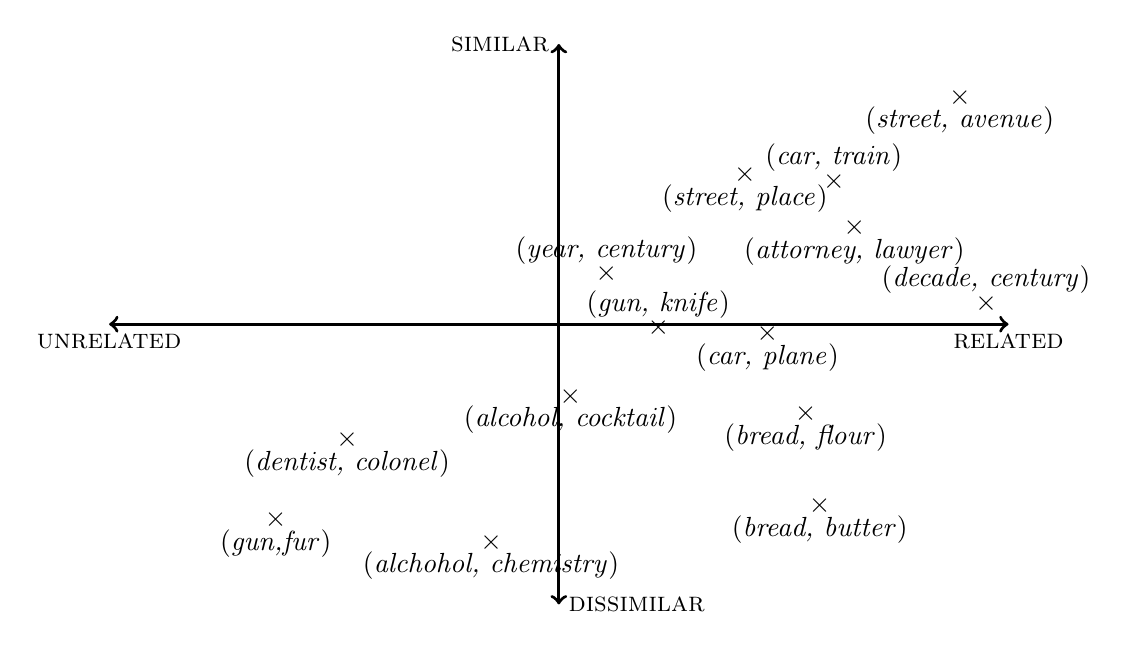
\begin{tikzpicture}
    \begin{axis}[xscale=2,yscale=1.5,hide axis]
      \addplot [<->,very thick] coordinates{(0,5) (10,5)};
      \addplot [<->,very thick] coordinates{(5,0) (5,10)};
      \node at (axis cs: 0,5) [below] {\normalsize \textsc{unrelated}};
      \node at (axis cs: 10,5) [below] {\normalsize \textsc{related}};
      \node at (axis cs: 5,0) [right] {\normalsize \textsc{dissimilar}};
      \node at (axis cs: 5,10) [left] {\normalsize \textsc{similar}};
      \node at (axis cs: 7.901,1.760) [below] {(\emph{bread, butter})};
      \node at (axis cs: 7.901,1.760) {$\times$};
      \node at (axis cs: 2.646,2.940) [below] {(\emph{dentist, colonel})};
      \node at (axis cs: 2.646,2.940) {$\times$};
      \node at (axis cs: 4.247,1.109) [below] {(\emph{alchohol, chemistry})};
      \node at (axis cs: 4.247,1.109) {$\times$};
      \node at (axis cs: 7.744,3.406) [below] {(\emph{bread, flour})};
      \node at (axis cs: 7.744,3.406) {$\times$};
      \node at (axis cs: 5.129,3.714) [below] {(\emph{alcohol, cocktail})};
      \node at (axis cs: 5.129,3.714) {$\times$};
      \node at (axis cs: 5.530,5.901) [above] {(\emph{year, century})};
      \node at (axis cs: 5.530,5.901) {$\times$};
      \node at (axis cs: 9.75,5.368) [above] {(\emph{decade, century})};
      \node at (axis cs: 9.75,5.368) {$\times$};
      \node at (axis cs: 7.320,4.828) [below] {(\emph{car, plane})};
      \node at (axis cs: 7.320,4.828) {$\times$};
      \node at (axis cs: 8.057,7.550) [above] {(\emph{car, train})};
      \node at (axis cs: 8.057,7.550) {$\times$};
      \node at (axis cs: 8.286,6.724) [below] {(\emph{attorney, lawyer})};
      \node at (axis cs: 8.286,6.724) {$\times$};
      \node at (axis cs: 1.852,1.512) [below] {(\emph{gun,fur})};
      \node at (axis cs: 1.852,1.512) {$\times$};
      \node at (axis cs: 6.106,4.936) [above] {(\emph{gun, knife})};
      \node at (axis cs: 6.106,4.936) {$\times$};
      \node at (axis cs: 7.068,7.667) [below] {(\emph{street, place})};
      \node at (axis cs: 7.068,7.667) {$\times$};
      \node at (axis cs: 9.458,9.050) [below] {(\emph{street, avenue})};
      \node at (axis cs: 9.458,9.050) {$\times$};
    \end{axis}
  \end{tikzpicture}
\caption{Noun pair scores along axes of relatedness and similarity as returned by a model built from features of 2x2 word co-occurrence window, 400 dimensional, \textsc{indy} type subspaces.}
\label{fig:axes}
\end{figure}

\footnote{Intriguingly, when identical words are given as input, they are rated as being very related and very dissimilar.  The latter outcome is obviously an imperfection, but it also reveals the extent to which the models of each type of semantic phenomenon are making use of different geometric features, or the same features in opposite ways.}

\begin{figure}
\footnotesize
\begin{subfigure}{0.3\textwidth} % alcohol - cocktail
\centering
  \begin{tikzpicture}
    \def\varA{79.0460,0.0100,36.6061};
    \def\varB{0.0100,84.4756,44.1699};
    \def\varC{30.1642,30.1641,30.1644};
    \def\varM{26.1589,22.2901,42.0425};
    \def\varX{54.3220,50.1692,92.1549};
    \def\varAN{27.2226,0.0035,12.6067};
    \def\varBN{0.0032,26.5852,13.9006};
    \def\varCN{17.3205,17.3204,17.3206};
    \def\varMN{14.4519,12.3145,23.2270};
    \def\varXN{13.7927,12.7383,23.3987};
    \begin{axis}[scale = 0.6,axis line style=white,view={120}{10},xmin=0,xmax=100,ymin=0,ymax=100,zmin=0,zmax=100,colormap/blackwhite,ticks=none]
      \addplot3[color=black,thick] coordinates {(0,0,100) (0,100,100)};
      \addplot3[color=black,thick] coordinates {(0,0,100) (100,0,100)};
      \addplot3[color=black,thick] coordinates {(0,100,0) (0,100,100)};
      \addplot3[color=black,thick] coordinates {(0,100,0) (100,100,0)};
      \addplot3[color=black,thick] coordinates {(100,0,0) (100,0,100)};
      \addplot3[color=black,thick] coordinates {(100,0,0) (100,100,0)};
      \addplot3[color=black] coordinates {(0,0,0) (0,0,100)};
      \addplot3[color=black] coordinates {(0,0,0) (0,100,0)};
      \addplot3[color=black] coordinates {(0,0,0) (100,0,0)};
      \addplot3[patch,patch type=triangle,color=gray,fill opacity=0.6] coordinates {(0.0,0.0,0.0) (\varCN) (\varAN)};
      \addplot3[patch,patch type=triangle,color=gray,fill opacity=0.5] coordinates {(0.0,0.0,0.0) (\varCN) (\varBN)};
      \addplot3[patch,patch type=triangle,color=darkgray,fill opacity=0.5] coordinates {(\varCN) (\varAN) (\varBN)};
      \addplot3 [color=black,thick] coordinates {(0,0,0) (\varCN)};
      \addplot3 [color=black,thick] coordinates {(0,0,0) (\varXN)};
      \addplot3 [color=black,thick] coordinates {(0,0,0) (\varMN)};
%      \addplot3[opacity = 0.1,surf,z buffer = sort,samples = 21,variable = \u,variable y = \v,domain = 0:90,y domain = 0:90,]
%    ({1*cos(u)*sin(v)}, {1*sin(u)*sin(v)}, {1*cos(v)});
      \addplot3 [patch,patch type=rectangle,color=lightgray,fill opacity=0.6] coordinates{(\varAN) (\varA) (\varB) (\varBN)
};
      \addplot3 [color=black,thick] coordinates {(\varCN) (\varC)};
      \addplot3 [color=black,thick] coordinates {(\varXN) (\varX)};
      \addplot3 [color=black,thick] coordinates {(\varMN) (\varM)};
      \addplot3 [patch,patch type=triangle,color=lightgray,fill opacity=0.6] coordinates{(\varA) (\varC) (\varB)};
      \addplot3 [patch,patch type=triangle,color=gray,fill opacity=0.8] coordinates{(\varA) (\varX) (\varB)};
      \addplot3 [patch,patch type=triangle,color=gray,fill opacity=0.6] coordinates{(\varA) (\varM) (\varB)};
%      \node [anchor=south] at (axis cs: 0.1,0.0,0.0) {O};
      \node [anchor=south] at (axis cs: \varA) {alcohol};
      \node [anchor=south] at (axis cs: \varB) {cocktail};
%      \node [anchor=south] at (axis cs: \varAN) {A'};
%      \node [anchor=west] at (axis cs: \varBN) {B'};
%      \node [anchor=south] at (axis cs: \varCN) {C'};
%      \draw plot [mark=*, mark size=1] coordinates{(axis cs: \varCN)};
      \node [anchor=south] at (axis cs: \varC) {C};
%      \node [anchor=east] at (axis cs: \varXN) {X'};
%      \draw plot [mark=*, mark size=1] coordinates{(axis cs: \varXN)};
      \node [anchor=south] at (axis cs: \varX) {X};
%      \node [anchor=west] at (axis cs: \varMN) {M'};
%      \draw plot [mark=*, mark size=1] coordinates{(axis cs: \varMN)};
      \node [anchor=south] at (axis cs: \varM) {M};
    \end{axis}
  \end{tikzpicture}
\caption*{\footnotesize \emph{relatedness = 5.129} \\ \emph{similarity = 3.714}}
\end{subfigure}
\hfill
\begin{subfigure}{0.3\textwidth} % year - century
\centering
  \begin{tikzpicture}
    \def\varA{51.9626,6.4671,21.7839};
    \def\varB{0.0100,63.1563,21.7575};
    \def\varC{25.6275,25.6274,25.6277};
    \def\varM{22.1142,19.2209,35.5466};
    \def\varX{51.7446,49.2619,82.4910};
    \def\varAN{27.4867,3.4209,11.5230};
    \def\varBN{0.0045,28.3640,9.7715};
    \def\varCN{17.3205,17.3204,17.3206};
    \def\varMN{14.4018,12.5175,23.1496};
    \def\varXN{14.2249,13.5424,22.6772};
    \begin{axis}[scale = 0.6,axis line style=white,view={120}{10},xmin=0,xmax=100,ymin=0,ymax=100,zmin=0,zmax=100,colormap/blackwhite,ticks=none]
      \addplot3[color=black,thick] coordinates {(0,0,100) (0,100,100)};
      \addplot3[color=black,thick] coordinates {(0,0,100) (100,0,100)};
      \addplot3[color=black,thick] coordinates {(0,100,0) (0,100,100)};
      \addplot3[color=black,thick] coordinates {(0,100,0) (100,100,0)};
      \addplot3[color=black,thick] coordinates {(100,0,0) (100,0,100)};
      \addplot3[color=black,thick] coordinates {(100,0,0) (100,100,0)};
      \addplot3[color=black] coordinates {(0,0,0) (0,0,100)};
      \addplot3[color=black] coordinates {(0,0,0) (0,100,0)};
      \addplot3[color=black] coordinates {(0,0,0) (100,0,0)};
      \addplot3[patch,patch type=triangle,color=gray,fill opacity=0.6] coordinates {(0.0,0.0,0.0) (\varCN) (\varAN)};
      \addplot3[patch,patch type=triangle,color=gray,fill opacity=0.5] coordinates {(0.0,0.0,0.0) (\varCN) (\varBN)};
      \addplot3[patch,patch type=triangle,color=darkgray,fill opacity=0.5] coordinates {(\varCN) (\varAN) (\varBN)};
      \addplot3 [color=black,thick] coordinates {(0,0,0) (\varCN)};
      \addplot3 [color=black,thick] coordinates {(0,0,0) (\varXN)};
      \addplot3 [color=black,thick] coordinates {(0,0,0) (\varMN)};
%      \addplot3[opacity = 0.1,surf,z buffer = sort,samples = 21,variable = \u,variable y = \v,domain = 0:90,y domain = 0:90,]
%    ({1*cos(u)*sin(v)}, {1*sin(u)*sin(v)}, {1*cos(v)});
      \addplot3 [patch,patch type=rectangle,color=lightgray,fill opacity=0.6] coordinates{(\varAN) (\varA) (\varB) (\varBN)
};
      \addplot3 [color=black,thick] coordinates {(\varCN) (\varC)};
      \addplot3 [color=black,thick] coordinates {(\varXN) (\varX)};
      \addplot3 [color=black,thick] coordinates {(\varMN) (\varM)};
      \addplot3 [patch,patch type=triangle,color=lightgray,fill opacity=0.6] coordinates{(\varA) (\varC) (\varB)};
      \addplot3 [patch,patch type=triangle,color=gray,fill opacity=0.8] coordinates{(\varA) (\varX) (\varB)};
      \addplot3 [patch,patch type=triangle,color=gray,fill opacity=0.6] coordinates{(\varA) (\varM) (\varB)};
%      \node [anchor=south] at (axis cs: 0.1,0.0,0.0) {O};
      \node [anchor=south] at (axis cs: \varA) {year};
      \node [anchor=south] at (axis cs: \varB) {century};
%      \node [anchor=south] at (axis cs: \varAN) {A'};
%      \node [anchor=west] at (axis cs: \varBN) {B'};
%      \node [anchor=south] at (axis cs: \varCN) {C'};
%      \draw plot [mark=*, mark size=1] coordinates{(axis cs: \varCN)};
      \node [anchor=south] at (axis cs: \varC) {C};
%      \node [anchor=east] at (axis cs: \varXN) {X'};
%      \draw plot [mark=*, mark size=1] coordinates{(axis cs: \varXN)};
      \node [anchor=south] at (axis cs: \varX) {X};
%      \node [anchor=west] at (axis cs: \varMN) {M'};
%      \draw plot [mark=*, mark size=1] coordinates{(axis cs: \varMN)};
      \node [anchor=south] at (axis cs: \varM) {M};
    \end{axis}
  \end{tikzpicture}
\caption*{\footnotesize \emph{relatedness = 5.530} \\ \emph{similarity = 5.901}}
\end{subfigure}
\hfill
\begin{subfigure}{0.3\textwidth} % car - train
\centering
  \begin{tikzpicture}
    \def\varA{19.9946,72.8400,15.5063};
    \def\varB{70.9042,15.2298,16.5710};
    \def\varC{28.8258,28.8259,28.8257};
    \def\varM{30.6877,33.1717,22.6174};
    \def\varX{70.4550,74.4422,58.8530};
    \def\varAN{7.7790,28.3389,6.0328};
    \def\varBN{28.5940,6.1418,6.6827};
    \def\varCN{17.3205,17.3206,17.3205};
    \def\varMN{18.2182,19.6929,13.4272};
    \def\varXN{17.8833,18.8953,14.9384};
%    \def\varA{19.9946,15.5063,72.8400};
%    \def\varB{70.9042,16.5710,15.2298};
%    \def\varC{28.8258,28.8257,28.8259};
%    \def\varM{30.6877,22.6174,33.1717};
%    \def\varX{70.4550,58.8530,74.4422};
%    \def\varAN{7.7790,6.0328,28.3389};
%    \def\varBN{28.5940,6.6827,6.1418};
%    \def\varCN{17.3205,17.3205,17.3206};
%    \def\varMN{18.2182,13.4272,19.6929};
%    \def\varXN{17.8833,14.9384,18.8953};
%    \def\varA{65.4685,49.1227,19.3840};
%    \def\varB{61.7135,61.5873,33.5169};
%    \def\varC{26.2133,26.2126,26.2126};
%    \def\varM{32.1238,32.7204,13.7926};
%    \def\varX{100.3424,50.3228,35.4999};
%    \def\varAN{23.3503,17.5204,6.9136};
%    \def\varBN{19.8208,19.7802,10.7648};
%    \def\varCN{17.3208,17.3203,17.3203};
%    \def\varMN{20.1264,20.5001,8.6414};
%    \def\varXN{25.5685,12.8229,9.0458};
%    \def\varA{49.1227,65.4685,19.3840};
%    \def\varB{61.5873,61.7135,33.5169};
%    \def\varC{26.2126,26.2133,26.2126};
%    \def\varM{32.7204,32.1238,13.7926};
%    \def\varX{50.3228,100.3424,35.4999};
%    \def\varAN{17.5204,23.3503,6.9136};
%    \def\varBN{19.7802,19.8208,10.7648};
%    \def\varCN{17.3203,17.3208,17.3203};
%    \def\varMN{20.5001,20.1264,8.6414};
%    \def\varXN{12.8229,25.5685,9.0458};
%    \def\varA{49.1227,19.3840,65.4685};
%    \def\varB{61.5873,33.5169,61.7135};
%    \def\varC{26.2126,26.2126,26.2133};
%    \def\varM{32.7204,13.7926,32.1238};
%    \def\varX{50.3228,35.4999,100.3424};
%    \def\varAN{17.5204,6.9136,23.3503};
%    \def\varBN{19.7802,10.7648,19.8208};
%    \def\varCN{17.3203,17.3203,17.3208};
%    \def\varMN{20.5001,8.6414,20.1264};
%    \def\varXN{12.8229,9.0458,25.5685};
    \begin{axis}[scale = 0.6,axis line style=white,view={120}{10},xmin=0,xmax=100,ymin=0,ymax=100,zmin=0,zmax=100,colormap/blackwhite,ticks=none]
      \addplot3[color=black,thick] coordinates {(0,0,100) (0,100,100)};
      \addplot3[color=black,thick] coordinates {(0,0,100) (100,0,100)};
      \addplot3[color=black,thick] coordinates {(0,100,0) (0,100,100)};
      \addplot3[color=black,thick] coordinates {(0,100,0) (100,100,0)};
      \addplot3[color=black,thick] coordinates {(100,0,0) (100,0,100)};
      \addplot3[color=black,thick] coordinates {(100,0,0) (100,100,0)};
      \addplot3[color=black] coordinates {(0,0,0) (0,0,100)};
      \addplot3[color=black] coordinates {(0,0,0) (0,100,0)};
      \addplot3[color=black] coordinates {(0,0,0) (100,0,0)};
      \addplot3[patch,patch type=triangle,color=gray,fill opacity=0.6] coordinates {(0.0,0.0,0.0) (\varCN) (\varAN)};
      \addplot3[patch,patch type=triangle,color=gray,fill opacity=0.5] coordinates {(0.0,0.0,0.0) (\varCN) (\varBN)};
      \addplot3[patch,patch type=triangle,color=darkgray,fill opacity=0.5] coordinates {(\varCN) (\varAN) (\varBN)};
      \addplot3 [color=black,thick] coordinates {(0,0,0) (\varCN)};
      \addplot3 [color=black,thick] coordinates {(0,0,0) (\varXN)};
      \addplot3 [color=black,thick] coordinates {(0,0,0) (\varMN)};
%      \addplot3[opacity = 0.1,surf,z buffer = sort,samples = 21,variable = \u,variable y = \v,domain = 0:90,y domain = 0:90,]
%    ({1*cos(u)*sin(v)}, {1*sin(u)*sin(v)}, {1*cos(v)});
      \addplot3 [patch,patch type=rectangle,color=lightgray,fill opacity=0.6] coordinates{(\varAN) (\varA) (\varB) (\varBN)
};
      \addplot3 [color=black,thick] coordinates {(\varCN) (\varC)};
      \addplot3 [color=black,thick] coordinates {(\varXN) (\varX)};
      \addplot3 [color=black,thick] coordinates {(\varMN) (\varM)};
      \addplot3 [patch,patch type=triangle,color=lightgray,fill opacity=0.6] coordinates{(\varA) (\varC) (\varB)};
      \addplot3 [patch,patch type=triangle,color=gray,fill opacity=0.8] coordinates{(\varA) (\varX) (\varB)};
      \addplot3 [patch,patch type=triangle,color=gray,fill opacity=0.6] coordinates{(\varA) (\varM) (\varB)};
%      \node [anchor=south] at (axis cs: 0.1,0.0,0.0) {O};
      \node [anchor=south] at (axis cs: \varA) {car};
      \node [anchor=south] at (axis cs: \varB) {train};
%      \node [anchor=south] at (axis cs: \varAN) {A'};
%      \node [anchor=west] at (axis cs: \varBN) {B'};
%      \node [anchor=south] at (axis cs: \varCN) {C'};
%      \draw plot [mark=*, mark size=1] coordinates{(axis cs: \varCN)};
      \node [anchor=south] at (axis cs: \varC) {C};
%      \node [anchor=east] at (axis cs: \varXN) {X'};
%      \draw plot [mark=*, mark size=1] coordinates{(axis cs: \varXN)};
      \node [anchor=south] at (axis cs: \varX) {X};
%      \node [anchor=west] at (axis cs: \varMN) {M'};
%      \draw plot [mark=*, mark size=1] coordinates{(axis cs: \varMN)};
      \node [anchor=south] at (axis cs: \varM) {M};
    \end{axis}
  \end{tikzpicture}
\caption*{\footnotesize \emph{relatedness = 8.057} \\ \emph{similarity = 7.550}}
\end{subfigure}
\vfill
\vspace{10pt}
\vfill
\begin{subfigure}{0.3\textwidth} % gun-fur
\centering
  \begin{tikzpicture}
    \def\varA{0.2227,83.1037,19.3450};
    \def\varB{80.6411,0.0100,24.3846};
    \def\varC{31.2668,31.2672,31.2669};
    \def\varM{36.2502,37.1321,20.4184};
    \def\varX{73.2282,78.5851,58.6705};
    \def\varAN{0.0783,29.2187,6.8016};
    \def\varBN{28.7159,0.0036,8.6832};
    \def\varCN{17.3204,17.3206,17.3205};
    \def\varMN{19.5015,19.9759,10.9844};
    \def\varXN{17.9490,19.2620,14.3808};
%    \def\varA{0.2227,19.3450,83.1037};
%    \def\varB{80.6411,24.3846,0.0100};
%    \def\varC{31.2668,31.2669,31.2672};
%    \def\varM{36.2502,20.4184,37.1321};
%    \def\varX{73.2282,58.6705,78.5851};
%    \def\varAN{0.0783,6.8016,29.2187};
%    \def\varBN{28.7159,8.6832,0.0036};
%    \def\varCN{17.3204,17.3205,17.3206};
%    \def\varMN{19.5015,10.9844,19.9759};
%    \def\varXN{17.9490,14.3808,19.2620};
    \begin{axis}[scale = 0.6,axis line style=white,view={120}{10},xmin=0,xmax=100,ymin=0,ymax=100,zmin=0,zmax=100,colormap/blackwhite,ticks=none]
      \addplot3[color=black,thick] coordinates {(0,0,100) (0,100,100)};
      \addplot3[color=black,thick] coordinates {(0,0,100) (100,0,100)};
      \addplot3[color=black,thick] coordinates {(0,100,0) (0,100,100)};
      \addplot3[color=black,thick] coordinates {(0,100,0) (100,100,0)};
      \addplot3[color=black,thick] coordinates {(100,0,0) (100,0,100)};
      \addplot3[color=black,thick] coordinates {(100,0,0) (100,100,0)};
      \addplot3[color=black] coordinates {(0,0,0) (0,0,100)};
      \addplot3[color=black] coordinates {(0,0,0) (0,100,0)};
      \addplot3[color=black] coordinates {(0,0,0) (100,0,0)};
      \addplot3[patch,patch type=triangle,color=gray,fill opacity=0.6] coordinates {(0.0,0.0,0.0) (\varCN) (\varAN)};
      \addplot3[patch,patch type=triangle,color=gray,fill opacity=0.5] coordinates {(0.0,0.0,0.0) (\varCN) (\varBN)};
      \addplot3[patch,patch type=triangle,color=darkgray,fill opacity=0.5] coordinates {(\varCN) (\varAN) (\varBN)};
      \addplot3 [color=black,thick] coordinates {(0,0,0) (\varCN)};
      \addplot3 [color=black,thick] coordinates {(0,0,0) (\varXN)};
      \addplot3 [color=black,thick] coordinates {(0,0,0) (\varMN)};
%      \addplot3[opacity = 0.1,surf,z buffer = sort,samples = 21,variable = \u,variable y = \v,domain = 0:90,y domain = 0:90,]
%    ({1*cos(u)*sin(v)}, {1*sin(u)*sin(v)}, {1*cos(v)});
      \addplot3 [patch,patch type=rectangle,color=lightgray,fill opacity=0.6] coordinates{(\varAN) (\varA) (\varB) (\varBN)
};
      \addplot3 [color=black,thick] coordinates {(\varCN) (\varC)};
      \addplot3 [color=black,thick] coordinates {(\varXN) (\varX)};
      \addplot3 [color=black,thick] coordinates {(\varMN) (\varM)};
      \addplot3 [patch,patch type=triangle,color=lightgray,fill opacity=0.6] coordinates{(\varA) (\varC) (\varB)};
      \addplot3 [patch,patch type=triangle,color=gray,fill opacity=0.8] coordinates{(\varA) (\varX) (\varB)};
      \addplot3 [patch,patch type=triangle,color=gray,fill opacity=0.6] coordinates{(\varA) (\varM) (\varB)};
%      \node [anchor=south] at (axis cs: 0.1,0.0,0.0) {O};
      \node [anchor=south] at (axis cs: \varA) {gun};
      \node [anchor=south] at (axis cs: \varB) {fur};
%      \node [anchor=south] at (axis cs: \varAN) {A'};
%      \node [anchor=west] at (axis cs: \varBN) {B'};
%      \node [anchor=south] at (axis cs: \varCN) {C'};
%      \draw plot [mark=*, mark size=1] coordinates{(axis cs: \varCN)};
      \node [anchor=south] at (axis cs: \varC) {C};
%      \node [anchor=east] at (axis cs: \varXN) {X'};
%      \draw plot [mark=*, mark size=1] coordinates{(axis cs: \varXN)};
      \node [anchor=south] at (axis cs: \varX) {X};
%      \node [anchor=west] at (axis cs: \varMN) {M'};
%      \draw plot [mark=*, mark size=1] coordinates{(axis cs: \varMN)};
      \node [anchor=south] at (axis cs: \varM) {M};
    \end{axis}
  \end{tikzpicture}
\caption*{\footnotesize \emph{relatedness = 1.852} \\ \emph{similarity = 1.512}}
\end{subfigure}
\hfill
\begin{subfigure}{0.3\textwidth} %alcohol - chemistry
\centering
  \begin{tikzpicture}
    \def\varA{6.2406,84.0428,11.2675};
    \def\varB{77.9932,3.0879,15.4691};
    \def\varC{30.4804,30.4805,30.4803};
    \def\varM{31.5977,34.8934,24.9498};
    \def\varX{70.7068,73.5172,59.2103};
    \def\varAN{2.2020,29.6538,3.9757};
    \def\varBN{29.4046,1.1642,5.8321};
    \def\varCN{17.3205,17.3206,17.3204};
    \def\varMN{17.7924,19.6482,14.0491};
    \def\varXN{17.9853,18.7002,15.0610};
%    \def\varA{6.2406,11.2675,84.0428};
%    \def\varB{77.9932,15.4691,3.0879};
%    \def\varC{30.4804,30.4803,30.4805};
%    \def\varM{31.5977,24.9498,34.8934};
%    \def\varX{70.7068,59.2103,73.5172};
%    \def\varAN{2.2020,3.9757,29.6538};
%    \def\varBN{29.4046,5.8321,1.1642};
%    \def\varCN{17.3205,17.3204,17.3206};
%    \def\varMN{17.7924,14.0491,19.6482};
%    \def\varXN{17.9853,15.0610,18.7002};
    \begin{axis}[scale = 0.6,axis line style=white,view={120}{10},xmin=0,xmax=100,ymin=0,ymax=100,zmin=0,zmax=100,colormap/blackwhite,ticks=none]
      \addplot3[color=black,thick] coordinates {(0,0,100) (0,100,100)};
      \addplot3[color=black,thick] coordinates {(0,0,100) (100,0,100)};
      \addplot3[color=black,thick] coordinates {(0,100,0) (0,100,100)};
      \addplot3[color=black,thick] coordinates {(0,100,0) (100,100,0)};
      \addplot3[color=black,thick] coordinates {(100,0,0) (100,0,100)};
      \addplot3[color=black,thick] coordinates {(100,0,0) (100,100,0)};
      \addplot3[color=black] coordinates {(0,0,0) (0,0,100)};
      \addplot3[color=black] coordinates {(0,0,0) (0,100,0)};
      \addplot3[color=black] coordinates {(0,0,0) (100,0,0)};
      \addplot3[patch,patch type=triangle,color=gray,fill opacity=0.6] coordinates {(0.0,0.0,0.0) (\varCN) (\varAN)};
      \addplot3[patch,patch type=triangle,color=gray,fill opacity=0.5] coordinates {(0.0,0.0,0.0) (\varCN) (\varBN)};
      \addplot3[patch,patch type=triangle,color=darkgray,fill opacity=0.5] coordinates {(\varCN) (\varAN) (\varBN)};
      \addplot3 [color=black,thick] coordinates {(0,0,0) (\varCN)};
      \addplot3 [color=black,thick] coordinates {(0,0,0) (\varXN)};
      \addplot3 [color=black,thick] coordinates {(0,0,0) (\varMN)};
%      \addplot3[opacity = 0.1,surf,z buffer = sort,samples = 21,variable = \u,variable y = \v,domain = 0:90,y domain = 0:90,]
%    ({1*cos(u)*sin(v)}, {1*sin(u)*sin(v)}, {1*cos(v)});
      \addplot3 [patch,patch type=rectangle,color=lightgray,fill opacity=0.6] coordinates{(\varAN) (\varA) (\varB) (\varBN)
};
      \addplot3 [color=black,thick] coordinates {(\varCN) (\varC)};
      \addplot3 [color=black,thick] coordinates {(\varXN) (\varX)};
      \addplot3 [color=black,thick] coordinates {(\varMN) (\varM)};
      \addplot3 [patch,patch type=triangle,color=lightgray,fill opacity=0.6] coordinates{(\varA) (\varC) (\varB)};
      \addplot3 [patch,patch type=triangle,color=gray,fill opacity=0.8] coordinates{(\varA) (\varX) (\varB)};
      \addplot3 [patch,patch type=triangle,color=gray,fill opacity=0.6] coordinates{(\varA) (\varM) (\varB)};
%      \node [anchor=south] at (axis cs: 0.1,0.0,0.0) {O};
      \node [anchor=south] at (axis cs: \varA) {alcohol};
      \node [anchor=south] at (axis cs: \varB) {chemistry};
%      \node [anchor=south] at (axis cs: \varAN) {A'};
%      \node [anchor=west] at (axis cs: \varBN) {B'};
%      \node [anchor=south] at (axis cs: \varCN) {C'};
%      \draw plot [mark=*, mark size=1] coordinates{(axis cs: \varCN)};
      \node [anchor=south] at (axis cs: \varC) {C};
%      \node [anchor=east] at (axis cs: \varXN) {X'};
%      \draw plot [mark=*, mark size=1] coordinates{(axis cs: \varXN)};
      \node [anchor=south] at (axis cs: \varX) {X};
%      \node [anchor=west] at (axis cs: \varMN) {M'};
%      \draw plot [mark=*, mark size=1] coordinates{(axis cs: \varMN)};
      \node [anchor=south] at (axis cs: \varM) {M};
    \end{axis}
  \end{tikzpicture}
\caption*{\footnotesize \emph{relatedness = 4.247} \\ \emph{similarity = 1.109}}
\end{subfigure}
\hfill
\begin{subfigure}{0.3\textwidth} %bread - butter
\centering
  \begin{tikzpicture}
    \def\varA{27.0584,98.9587,33.0727};
    \def\varB{100.9304,27.8853,38.9284};
    \def\varC{31.8889,31.8891,31.8889};
    \def\varM{37.0303,37.7084,20.9277};
    \def\varX{72.6366,77.1240,57.5067};
    \def\varAN{7.5308,27.5420,9.2047};
    \def\varBN{27.1042,7.4884,10.4540};
    \def\varCN{17.3205,17.3206,17.3205};
    \def\varMN{19.5434,19.9013,11.0450};
    \def\varXN{18.0770,19.1938,14.3116};
%    \def\varA{27.0584,33.0727,98.9587};
%    \def\varB{100.9304,38.9284,27.8853};
%    \def\varC{31.8889,31.8889,31.8891};
%    \def\varM{37.0303,20.9277,37.7084};
%    \def\varX{72.6366,57.5067,77.1240};
%    \def\varAN{7.5308,9.2047,27.5420};
%    \def\varBN{27.1042,10.4540,7.4884};
%    \def\varCN{17.3205,17.3205,17.3206};
%    \def\varMN{19.5434,11.0450,19.9013};
%    \def\varXN{18.0770,14.3116,19.1938};
    \begin{axis}[scale = 0.6,axis line style=white,view={120}{10},xmin=0,xmax=100,ymin=0,ymax=100,zmin=0,zmax=100,colormap/blackwhite,ticks=none]
      \addplot3[color=black,thick] coordinates {(0,0,100) (0,100,100)};
      \addplot3[color=black,thick] coordinates {(0,0,100) (100,0,100)};
      \addplot3[color=black,thick] coordinates {(0,100,0) (0,100,100)};
      \addplot3[color=black,thick] coordinates {(0,100,0) (100,100,0)};
      \addplot3[color=black,thick] coordinates {(100,0,0) (100,0,100)};
      \addplot3[color=black,thick] coordinates {(100,0,0) (100,100,0)};
      \addplot3[color=black] coordinates {(0,0,0) (0,0,100)};
      \addplot3[color=black] coordinates {(0,0,0) (0,100,0)};
      \addplot3[color=black] coordinates {(0,0,0) (100,0,0)};
      \addplot3[patch,patch type=triangle,color=gray,fill opacity=0.6] coordinates {(0.0,0.0,0.0) (\varCN) (\varAN)};
      \addplot3[patch,patch type=triangle,color=gray,fill opacity=0.5] coordinates {(0.0,0.0,0.0) (\varCN) (\varBN)};
      \addplot3[patch,patch type=triangle,color=darkgray,fill opacity=0.5] coordinates {(\varCN) (\varAN) (\varBN)};
      \addplot3 [color=black,thick] coordinates {(0,0,0) (\varCN)};
      \addplot3 [color=black,thick] coordinates {(0,0,0) (\varXN)};
      \addplot3 [color=black,thick] coordinates {(0,0,0) (\varMN)};
%      \addplot3[opacity = 0.1,surf,z buffer = sort,samples = 21,variable = \u,variable y = \v,domain = 0:90,y domain = 0:90,]
%    ({1*cos(u)*sin(v)}, {1*sin(u)*sin(v)}, {1*cos(v)});
      \addplot3 [patch,patch type=rectangle,color=lightgray,fill opacity=0.6] coordinates{(\varAN) (\varA) (\varB) (\varBN)
};
      \addplot3 [color=black,thick] coordinates {(\varCN) (\varC)};
      \addplot3 [color=black,thick] coordinates {(\varXN) (\varX)};
      \addplot3 [color=black,thick] coordinates {(\varMN) (\varM)};
      \addplot3 [patch,patch type=triangle,color=lightgray,fill opacity=0.6] coordinates{(\varA) (\varC) (\varB)};
      \addplot3 [patch,patch type=triangle,color=gray,fill opacity=0.8] coordinates{(\varA) (\varX) (\varB)};
      \addplot3 [patch,patch type=triangle,color=gray,fill opacity=0.6] coordinates{(\varA) (\varM) (\varB)};
%      \node [anchor=south] at (axis cs: 0.1,0.0,0.0) {O};
      \node [anchor=south] at (axis cs: \varA) {bread};
      \node [anchor=south] at (axis cs: \varB) {butter};
%      \node [anchor=south] at (axis cs: \varAN) {A'};
%      \node [anchor=west] at (axis cs: \varBN) {B'};
%      \node [anchor=south] at (axis cs: \varCN) {C'};
%      \draw plot [mark=*, mark size=1] coordinates{(axis cs: \varCN)};
      \node [anchor=south] at (axis cs: \varC) {C};
%      \node [anchor=east] at (axis cs: \varXN) {X'};
%      \draw plot [mark=*, mark size=1] coordinates{(axis cs: \varXN)};
      \node [anchor=south] at (axis cs: \varX) {X};
%      \node [anchor=west] at (axis cs: \varMN) {M'};
%      \draw plot [mark=*, mark size=1] coordinates{(axis cs: \varMN)};
      \node [anchor=south] at (axis cs: \varM) {M};
    \end{axis}
  \end{tikzpicture}
\caption*{\footnotesize \emph{relatedness = 7.901} \\ \emph{similarity = 1.760}}
\end{subfigure}
\end{figure}

\section{Frames of Similarity} \label{sec:frames}
\cite{Tversky1977}, in his psychologically motivated reflections on the geometry of similarity, observes that relationships of similarity are fundamentally not symmetric: 

(for comparison, see where the pair (\emph{dentist, colonel}) falls in the space of Figure~\ref{fig:axes}, where it is one of the very few pairs considered to be marginally more similar than related)
